\documentclass[tikz,border=15pt]{standalone}
\usepackage{tikz}
\usetikzlibrary{shapes.geometric, arrows.meta, positioning}

\tikzset{
    register/.style={
        rectangle, draw=black, thick,
        minimum width=1.3cm, minimum height=0.9cm,
        fill=white, font=\small\ttfamily
    },
    mux/.style={
        trapezium, trapezium left angle=70, trapezium right angle=110,
        draw=black, thick,
        minimum width=1cm, minimum height=0.8cm,
        fill=white, font=\small
    },
    memory/.style={
        rectangle, draw=black, very thick,
        minimum width=1.5cm, minimum height=0.95cm,
        fill=white, font=\small
    },
    wire/.style={draw=black, thick, -Stealth},
    bus/.style={draw=black, line width=1.8pt, -Stealth},
    buswidth/.style={font=\scriptsize, fill=white, inner sep=2pt},
    logic/.style={
        rectangle, draw=black, thick, rounded corners=3pt,
        minimum width=1.2cm, minimum height=0.85cm,
        fill=gray!10, font=\small
    },
    sbox/.style={
        rectangle, draw=black, thick,
        minimum width=0.75cm, minimum height=0.75cm,
        fill=gray!20, font=\small
    }
}

\begin{document}
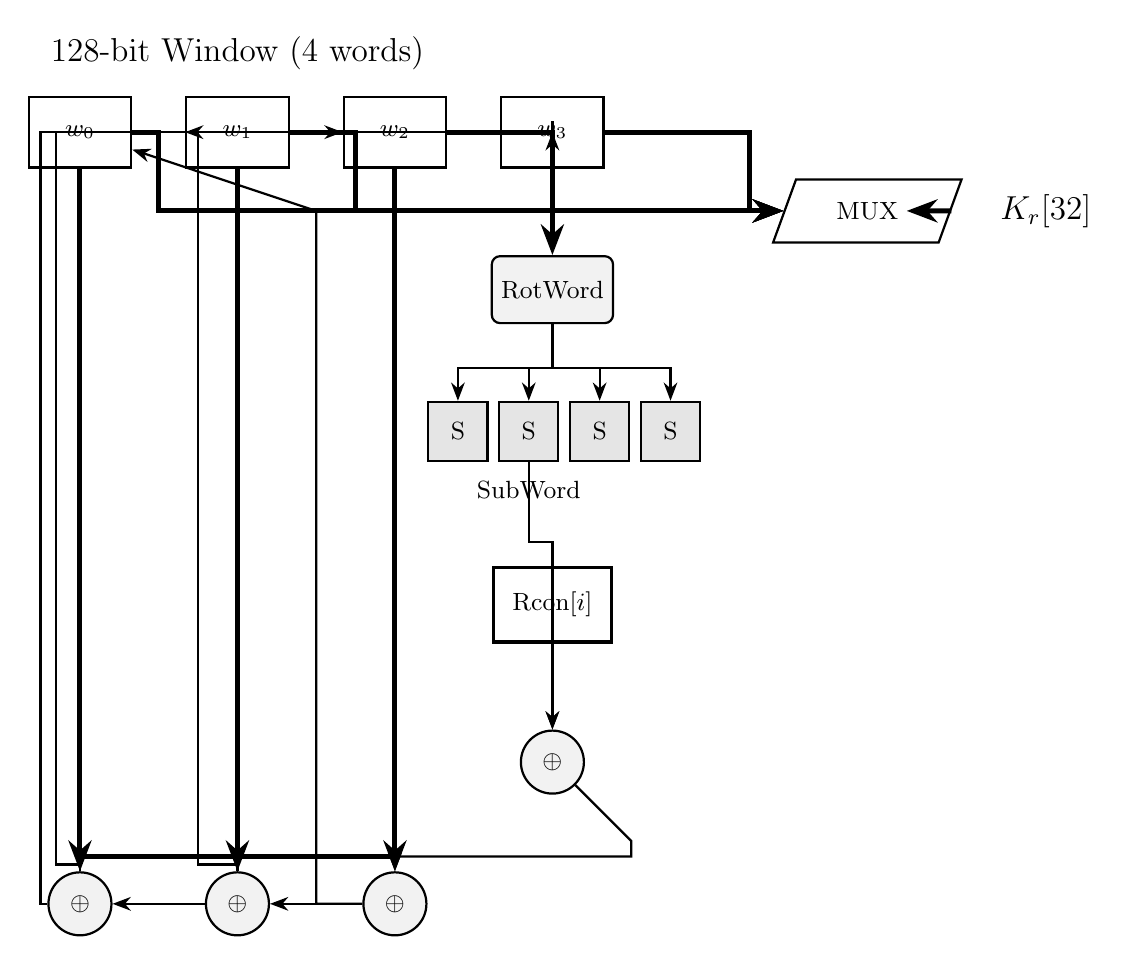
\begin{tikzpicture}

% Top row: 4-word window
\node[register] (w0) at (0,8) {$w_0$};
\node[register] (w1) at (2,8) {$w_1$};
\node[register] (w2) at (4,8) {$w_2$};
\node[register] (w3) at (6,8) {$w_3$};

\node[font=\large, above=0.2cm of w1.north] {128-bit Window (4 words)};

% RotWord
\node[logic] (rot) at (6,6) {RotWord};

% SubWord S-boxes
\node[sbox] (s0) at (4.8,4.2) {S};
\node[sbox] (s1) at (5.7,4.2) {S};
\node[sbox] (s2) at (6.6,4.2) {S};
\node[sbox] (s3) at (7.5,4.2) {S};
\node[font=\small, below=0.12cm of s1.south] {SubWord};

% Rcon
\node[memory] (rcon) at (6,2) {Rcon[$i$]};

% XOR chain
\node[logic, circle, minimum size=0.8cm] (x1) at (6,0) {$\oplus$};
\node[logic, circle, minimum size=0.8cm] (x2) at (4,-1.8) {$\oplus$};
\node[logic, circle, minimum size=0.8cm] (x3) at (2,-1.8) {$\oplus$};
\node[logic, circle, minimum size=0.8cm] (x4) at (0,-1.8) {$\oplus$};

% Connections
\draw[bus] (w3) -- (rot);
\draw[wire] (rot) -- ++(0,-1) -| (s0);
\draw[wire] (rot) -- ++(0,-1) -| (s1);
\draw[wire] (rot) -- ++(0,-1) -| (s2);
\draw[wire] (rot) -- ++(0,-1) -| (s3);

\draw[wire] (s1) -- ++(0,-1.4) -| (x1);
\draw[wire] (rcon) -- (x1);
\draw[bus] (w0) -- ++(0,-9.2) -| (x2);
\draw[wire] (x1) -- ++(1,-1) -- ++(0,-0.2) -- ++(-3,0) -- (x2);
\draw[wire] (x2) -- (x3);
\draw[bus] (w1) -- ++(0,-9.2) -| (x3);
\draw[wire] (x3) -- (x4);
\draw[bus] (w2) -- ++(0,-9.2) -| (x4);

% Feedback paths
\draw[wire] (x2) -- ++(-1,0) -- ++(0,8.8) -- (w0);
\draw[wire] (x3) -- ++(0,0.5) -- ++(-0.5,0) -- ++(0,9.3) -- (w1);
\draw[wire] (x4) -- ++(0,0.5) -- ++(-0.3,0) -- ++(0,9.3) -- (w2);
\draw[wire] (x4) -- ++(-0.5,0) -- ++(0,9.8) -- ++(6.5,0) -- (w3);

% Output MUX
\node[mux] (outmux) at (10,7) {MUX};
\draw[bus] (w0) -- ++(1,0) |- (outmux);
\draw[bus] (w1) -- ++(1.5,0) |- (outmux);
\draw[bus] (w2) -- ++(2,0) |- (outmux);
\draw[bus] (w3) -- ++(2.5,0) |- (outmux);

\node[font=\large, right=0.5cm of outmux] {$K_r$[32]};
\draw[bus] (outmux) -- ++(0.5,0);

\end{tikzpicture}
\end{document}
